%%%%%%%%%%%%%%%%%%%%%%%%%%%%%%%%%%%%%%%%%
% Journal Article
% LaTeX Template
% Version 1.3 (9/9/13)
%
% This template has been downloaded from:
% http://www.LaTeXTemplates.com
%
% Original author:
% Frits Wenneker (http://www.howtotex.com)
%
% License:
% CC BY-NC-SA 3.0 (http://creativecommons.org/licenses/by-nc-sa/3.0/)
%
%%%%%%%%%%%%%%%%%%%%%%%%%%%%%%%%%%%%%%%%%

%----------------------------------------------------------------------------------------
%	PACKAGES AND OTHER DOCUMENT CONFIGURATIONS
%----------------------------------------------------------------------------------------

\documentclass[11pt]{article}

\usepackage[sc]{mathpazo} % Use the Palatino font
\usepackage[utf8]{inputenc}
\usepackage[T1]{fontenc} % Use 8-bit encoding that has 256 glyphs
\linespread{1.05} % Line spacing - Palatino needs more space between lines
\usepackage{microtype} % Slightly tweak font spacing for aesthetics

%\usepackage[hmarginratio=1:1,top=32mm,columnsep=20pt]{geometry} % Document margins
%\usepackage{multicol} % Used for the two-column layout of the document
\usepackage[hang, small,labelfont=bf,up,textfont=it,up]{caption} % Custom captions under/above floats in tables or figures
\usepackage{booktabs} % Horizontal rules in tables
\usepackage{float} % Required for tables and figures in the multi-column environment - they need to be placed in specific locations with the [H] (e.g. \begin{table}[H])
\usepackage[hidelinks]{hyperref} % For hyperlinks in the PDF

\usepackage{lettrine} % The lettrine is the first enlarged letter at the beginning of the text
%\usepackage{paralist} % Used for the compactitem environment which makes bullet points with less space between them

\usepackage{todonotes}
\usepackage{amsmath,amssymb,amsfonts}
\usepackage{subcaption}
\providecommand{\abs}[1]{\left \lvert #1 \right \rvert}

\usepackage{abstract} % Allows abstract customization
\renewcommand{\abstractnamefont}{\normalfont\bfseries} % Set the "Abstract" text to bold
\renewcommand{\abstracttextfont}{\normalfont\small\itshape} % Set the abstract itself to small italic text

\usepackage{titlesec} % Allows customization of titles
\renewcommand\thesection{\Roman{section}} % Roman numerals for the sections
\renewcommand\thesubsection{\Roman{subsection}} % Roman numerals for subsections
\titleformat{\section}[block]{\large\scshape\centering}{\thesection.}{1em}{} % Change the look of the section titles
\titleformat{\subsection}[block]{\large}{\thesubsection.}{1em}{} % Change the look of the section titles

\usepackage{fancyhdr} % Headers and footers
\pagestyle{fancy} % All pages have headers and footers
\fancyhead{} % Blank out the default header
\fancyfoot{} % Blank out the default footer
%\fancyhead[C]{Running title $\bullet$ November 2012 $\bullet$ Vol. XXI, No. 1} % Custom header text
\fancyfoot[RO,LE]{\thepage} % Custom footer text

%----------------------------------------------------------------------------------------
%	TITLE SECTION
%----------------------------------------------------------------------------------------

\title{\vspace{-15mm}\fontsize{24pt}{10pt}\selectfont\textbf{Local Adaptive
Optimization of Time Step}} % Article title

\author{
\large
\textsc{Malte Stær Nissen}\thanks{Thanks to my supervisor Sune Darkner for
helping me realize this project}\\[2mm] % Your name
\normalsize University of Copenhagen \\ % Your institution
\normalsize \href{mailto:nissen@diku.dk}{nissen@diku.dk} % Your email address
\vspace{-5mm}
}
\date{}

%----------------------------------------------------------------------------------------

\begin{document}

\maketitle % Insert title

\thispagestyle{fancy} % All pages have headers and footers

%----------------------------------------------------------------------------------------
%	ABSTRACT
%----------------------------------------------------------------------------------------

%\begin{abstract}


%\end{abstract}

%----------------------------------------------------------------------------------------
%	ARTICLE CONTENTS
%----------------------------------------------------------------------------------------

%\begin{multicols}{2} % Two-column layout throughout the main article text

\section{Introduction}
\lettrine[nindent=0em,lines=3]{S} imulations of large hyperelastic materials
can be very time consuming. When working with materials of varying density
of vertices/scale of mesh, the highest densities often give the most
strict bounds on size of the time step of the simulation in order to keep
the materials (and grids) stable and the discretization correct.

In a ``standard'' simulation with a global time step size we need to compute
possibly unnecessarily many computations on the coarser parts of the material
caused by this bound. When furthermore having materials with a large amount
of somewhat equally distributed vertices and smaller patches of detailed
areas with higher density of vertices, it would be an advantage to be able
to perform large time steps for the majority of the material (the coarse
parts) and smaller steps for the local patches where vertices could cause
instability. We call the concept of varying the timestep local adaptive
optimization of time step (LAOTS), in which ``local'' either refers to spatial
locality (as described above) or time locality where the time step is global
for all vertices but varies during the simulation.

We will in this report
study possible approaches for application of LAOTS. In order to keep the focus
on possible LAOTS methods and remove unneccessary complexities, we will study
the simple 1 dimensional simulation of a mass-spring system and try to apply
LAOTS for it. Afterwards we will shortly discuss the application of our gained
knowledge to the domain of hyperelastic material simulation and simulations in
general.

%------------------------------------------------

\section{Previous work} According to \cite{Gander:2013} local time stepping
was first studied in the community of ordinary differential equations (ODE)
with Rice \cite{rice:1960} developing the split Runge-Kutta methods (multi
rate Runge-Kutta methods). The concept behind these methods is the splitting
of the ODEs into multiple (two components in \cite{rice:1960}) components of
which each component needs to be integrated in different scales. A strategy
is chosen as proposed in \cite{Kvaernoe:1999} of either computing the coarser
part first (``Fastest first strategy'') followed by the finer part or vice
versa (``Slowest first strategy''). In order to perform these sequential
computations either interpolation or extrapolation of the first computation
is performed to compute the second part in each time step. The different
time step sizes can be adapted to fit the model in each step as well. See
\cite{Kvaernoe:1999} and \cite{Gear:1984} (similar strategy for linear multi
step methods) for more detailed descriptions of the two strategies.

In the partial differential equations (PDE) community, the adaptive time
stepping area was explored and developed with the goal of simulating
very specific known problems such as the (hyperbolic) wave equations
and (parabolic) heat equations instead of more general applications. We
will refrain from describing the methods further in this report, but a
short description and comparison of the specific methods can be found in
\cite{Gander:2013}. Generally the methods developed at first all make use
of the same basic concepts for making the local adaptive time stepping:
Interpolation, extrapolation, prediction and correction, which we are going to
use in the work of this report as well.

Recently newer and faster methods with local time stepping have been developed
on the basis of nonlinear PDEs and the work performed in this field in
the 80s and 90s. First the multi resolution (MR) schemes for creating
space-adaptive discretizations and refinements of these were developed, see
\cite{Berger:1984}. Then multiple MR based schemes were developed. Domingues
et al. \cite{Domingues:2008} is one of the more recent of these MR schemes.
They describe a local scale-dependent time stepping for a space-adaptive multi
resolution scheme using the finite volume method in order to obtain speed-up
using larger time-steps without violating a defined stability constraints,
which is essentially the same motivation as this report. The method is based
on an explicit Runge-Kutta method of second order. As expected the time step
size is imposed by a stability condition of the explicit Runge-Kutta on the
finest scale, which increases with the scale of the mesh and hence we are able
to increase the time step as well without violating the stability condition.


%------------------------------------------------

\section{Methods}
\label{sec:methods}

With no prerequisites within the field of mass simulations we will first
consider the 1D problem of simulating a mass-spring system using the explicit
(forward) Euler method.

Second we will propose and test out three different methods for applying LAOTS
to the simulation.

Third and last we will discussion the results and how we could apply our
knowledge of LAOTS for hyperelastic material.

\subsection{1D mass-spring system} Mass-spring systems are systems simulating
a set of vertices interconnected by springs in various ways to obtain
desirable physical properties. The motion of the springs and vertices are
then simulated as a function of the time elapsed. Examples of application of
mass-spring systems are simulation of cloth or hair. When performing simulations
we want to avoid a switch of position of spring-connected vertices caused by the
timestep size of the simulation, since this invalidates our discretization of
the domain. Furthermore we want to perform as few timesteps as possible in order
to get to the final simulation state by using as big timesteps as possible
without affecting the outcome of the simulation.

When simulating the mass-spring system we perform the following steps:
\begin{enumerate} \item Initialize system \item Calculate forces \item
Calculate derrivatives \item Update positions and velocities \item Update time
\item Go to step 2 if the simulation has not reached it's maximum simulation
time. \end{enumerate} We now describe the details of each of the steps of
the simulation.

Our 1D mass-spring system consists of a set $V$ of vertices and a set
$S$ of springs. Each vertex $v \in V$ has a specified position $p_v$,
mass $m_v$, force $F_v$ and velocity $u_v$, and each spring $s \in S$
has two endpoints vertices $p_{f,s} \in V$ and $p_{t,s} \in V \setminus
p_{f,s}$, a damping factor $d_s$, a stiffness constant $K_s$ and a rest length
$l_{0,s}$. All these variables and constants combined describe the state
of the mass-spring system at each time $t$ during a simulation. All these
variables are initialized in step 1.

The total force of a spring is the sum of the spring force $F_{h,d}$
calculated by using Hooke's Law (see \cite[p.~439]{Young:2010})
and the damping force $F_{C,d}$ using a simple damping method (see
\cite[p.~457]{Young:2010}): \begin{align} \nonumber l_d &= p_{l,d} -
p_{r,d} \\ \label{eq:hooke} F_{h,d} &= -k_d x_d = -k_d (l_d - l_{0,d}) \\
\label{eq:damping} F_{C,d} &= -C_d \frac{\partial x_d}{ \partial t} = - C_d
\frac{\left(v_{l,d} - v_{r,d}\right) l_d}{\abs{l_d}} \\ F_d &= F_{h,d} +
F_{C,d} \end{align} \todo{Maybe add direction correction: $F_d \cdot (-l_d
/ \abs{l_d})$} in which $p_{l,d}$ and $p_{r,d}$ are the positions of the
left and right endpoints of the spring $d$ respectively, and $v_{l,d}$ and
$v_{r,d}$ are the velocities of the left and right endpoint vertices of the
spring $d$ respectively, and $F_d$ is the total force of spring $d$.

When calculating the forces applied by each spring, we add the total spring
force $F_d$ to the left endpoint of the spring and subtract $F_d$ from the
right endpoint since both endpoints are affected equally in opposite direction
by the spring $d$ connecting them. These spring forces are calculated in step
2 of the simulation.

We now know how to calculate the force of the spring system and apply it to
the vertices. In order to calculate the derrivatives of the system (step 3) we
use Newton's second law of motion (see \cite[p.~112-115]{Young:2010}) to get
the difference in speed $\Delta u_v$ and position $\Delta p_v$ of each vertex
$v$ using a given time step size $\Delta t$: \begin{align} \label{eq:delta_u}
\Delta u_v &= \frac{\partial u_v}{\partial t} \Delta t = \frac{F_v}{m_v}
\Delta t \\ \label{eq:delta_p} \Delta p_v &= u \Delta t \end{align}

As mentioned in the beginning of this section we have chosen to use the
explicit Euler method defined below in equation \ref{eq:explicit_euler}
to calculate the time ``integration'' \cite{Flaherty} when stepping through
the simulation. Given a variable $x$ as a function of the time $t$, the
variable $x$ at the time $t + \Delta t$ is defined as: \begin{align}
\label{eq:explicit_euler} x(t+\Delta t) &= x(t) + \Delta t \frac{\partial
x(t)}{\partial t} \end{align} Applying this method for the timestepping
of our simulation we get the two following position and velocity update
equations using equations \ref{eq:delta_u} and \ref{eq:delta_p}: \begin{align}
p_v(t+\Delta t) &= p_v(t) + \Delta p_v \\ u_v(t+\Delta t) &= u_v(t) + \Delta
u_v \end{align} We use these equations to perform step 4 of the simulation.

Step 5 is a simple update of the time: $t = t + \Delta t$ and step 6 describes
itself.

We have now fully described the simple case of simulating a mass-spring system
using the explicit Euler method and the next subsections describe the three
different methods/modifications for applying LAOTS to the simulation just
described.

\subsection{Adapt-on-switch}
The first LAOT method we propose is time-adaptive. We perform a simulation
with an initial timestep size. In each step we try to predict whether a timestep
of the same size using the current velocities will result in a switch of the
left and right vertices of any of the springs. If this is the case, we should
try to avoid the switch by decreasing the timestep of the current iteration,
re-calculate the velocity and position changes and resume stepping of the
simulation using the new timestep size. When switches aren't detected anymore
we gradually increase the timestep of the simulation again. We call this
method the adapt-on-switch method.

The switch of two endspoints connected by a spring $d$ can easily be
calculated by checking the length ($p_{l,d} - p_{r,d}$) of the spring before
and after a position update. If the sign of the length differs, the two
points must have switched sides and hence adaption of the timestep should be
performed. The adaption of the timestep can either be done by division of the
current timestep by a constant or by having a finite set of timestep sizes to
choose from.

\subsection{Atomic updating using heuristics}
The second LAOT method we propose is space-adaptive. We perform simulations
using a fixed timestep size. In each iteration we perform position update of
all vertices, but only re-calculate acceleration and velocity of the springs
and points that fulfill some defined heuristics.

The heuristics can be chosen to fit the domain of the simulation, but we have
chosen to use the number of steps since last update and the ratio between the
current spring length and the spring length at the last update. This should
force a bound on the maximal timestep before update as well as making sure
updates are done more frequently in case the springlength is changing more
rapidly. Further details are explained in section \ref{sec:experiments}.

\subsection{Global estimated acceleration}
The third and last LAOT method we propose is time-adaptive. The simulations are
done using an initial timestep size. We know that the force and hence
acceleration of a spring is somewhat linear close to the spring's rest length
and it ``bends'' off as the spring is streched or contracted further away from
the rest length. Based on this knowledge we will try to make a heuristic
telling us about the needed timestep size at any given point during the
simulation. The smallest needed timestep defines the global timestep for that
given step.

For this simple 1D example we use the inverse of the acceleration
for adapting the timestep and hence the heuristic is defined as:
\begin{align}
    \frac{1}{a} &= \frac{1}{\frac{-kx}{m}} = \frac{m}{-kx} \\
    \Delta t &= \text{min}\left( \frac{1}{\abs{a} + 0.1} \right )
\end{align}
We have added a small value (0.1) in order to avoid the timestep to increase
exponentially towards infinity as $\abs{a}$ approach 0. Furthermore a scaling
of the timestep could be needed depending on the scale of the simulation mesh.
Further details are explained in section \ref{sec:experiments}.

Our though is that for some more
complex simulations we are able to make estimates of this type less costly than
performing the actual simulations of a small fixed size timestep.

%------------------------------------------------

\section{Experiments and results}
\label{sec:experiments}

We first give an example of the actual application of LAOTS using the standard
simulation of mass spring particles. Figure \ref{fig:std} shows two simulations
of the same set of particles distributed with two different scales simulated for
500 seconds each. All the springs $s \in S$ are initiated in a stretched state/position
with a length 1.25 times longer than the rest length, damping and stiffness
constants $C_s = 0.5, K_s = 0.5$, and all vertices $v \in V$
have a mass of $m_v = 30$.
\ref{fig:std_multi_30fps} shows a simulation using 30 fps and Figure
\ref{fig:std_multi_1fps} shows a simulation using 1 fps. We clearly see that
using a timestep of 30 fps the simulation is stable and able to handle the
compression of all the small springs around $t = 110$ whereas a switch occurs
when simulating at 1 fps. This switch causes ripples of sideeffects for the rest
of the simulation and hence the final result is incorrect. No switches of the longer springs are however occuring and hence these pose no problem at 1 fps. We will use this simulation for
testing all three LAOTS methods proposed in section \ref{sec:methods}.

\begin{figure}[H]
    \begin{subfigure}{0.5\textwidth}
        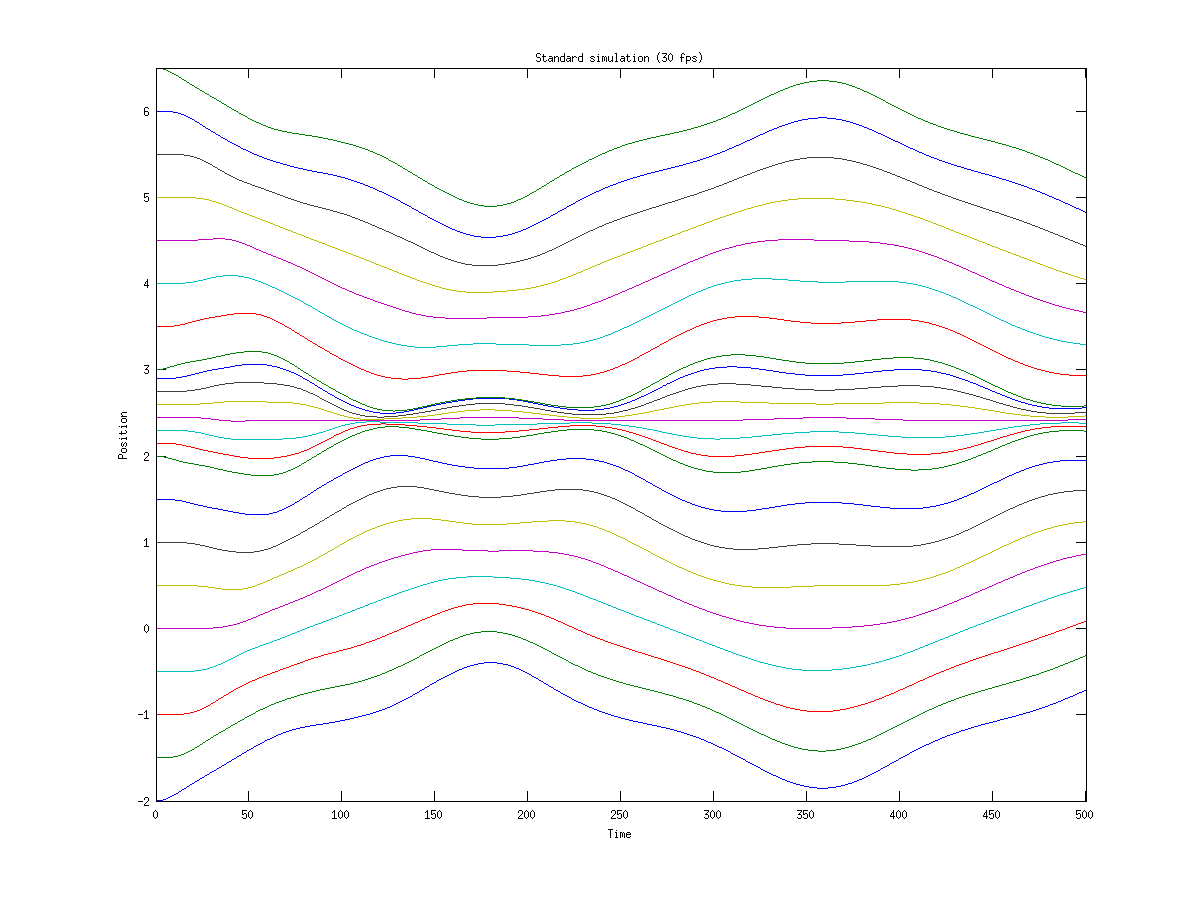
\includegraphics[width=\textwidth]{../images/standard_multiscale_30fps.png}
        \caption{30 fps}
        \label{fig:std_multi_30fps}
    \end{subfigure}
    \begin{subfigure}{0.5\textwidth}
        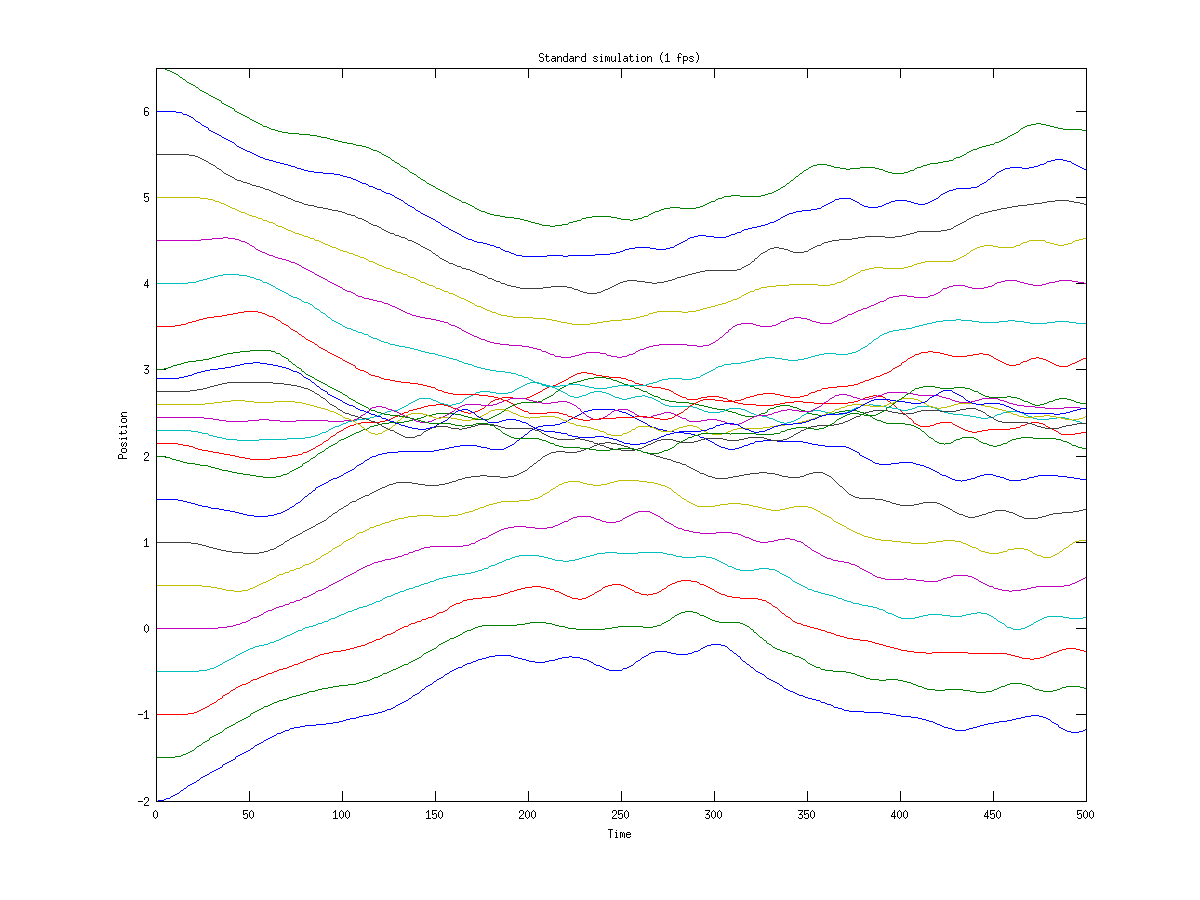
\includegraphics[width=\textwidth]{../images/standard_multiscale_1fps.png}
        \caption{1 fps}
        \label{fig:std_multi_1fps}
    \end{subfigure}
    \caption{Standard simulations of particles distributed with two scales using
    different timestep sizes}
    \label{fig:std}
\end{figure}

\todo{Write something about the explicit euler based on uniform}
\begin{figure}[H]
    \begin{subfigure}{0.5\textwidth}
        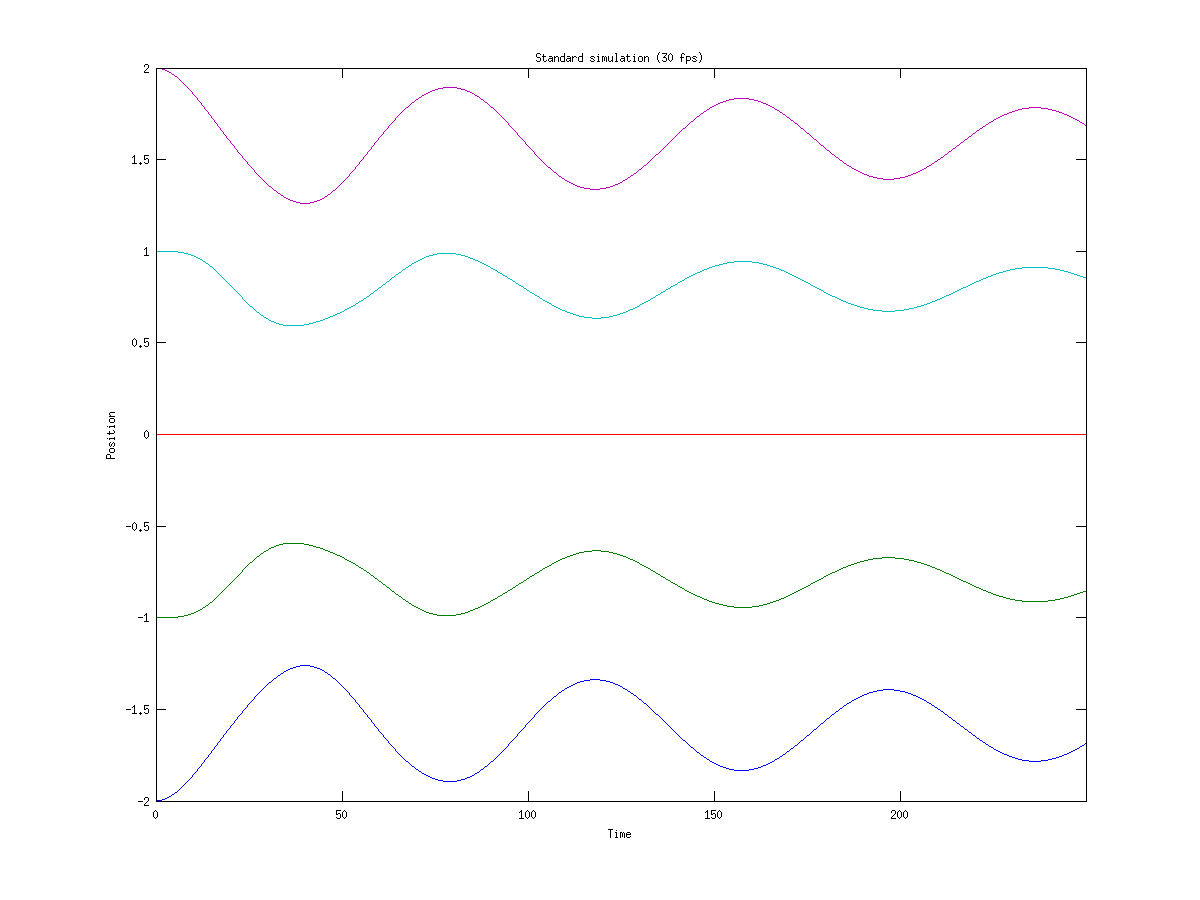
\includegraphics[width=\textwidth]{../images/standard_uniform_30fps.png}
        \caption{30 fps}
        \label{fig:std_uni_30fps}
    \end{subfigure}
    \begin{subfigure}{0.5\textwidth}
        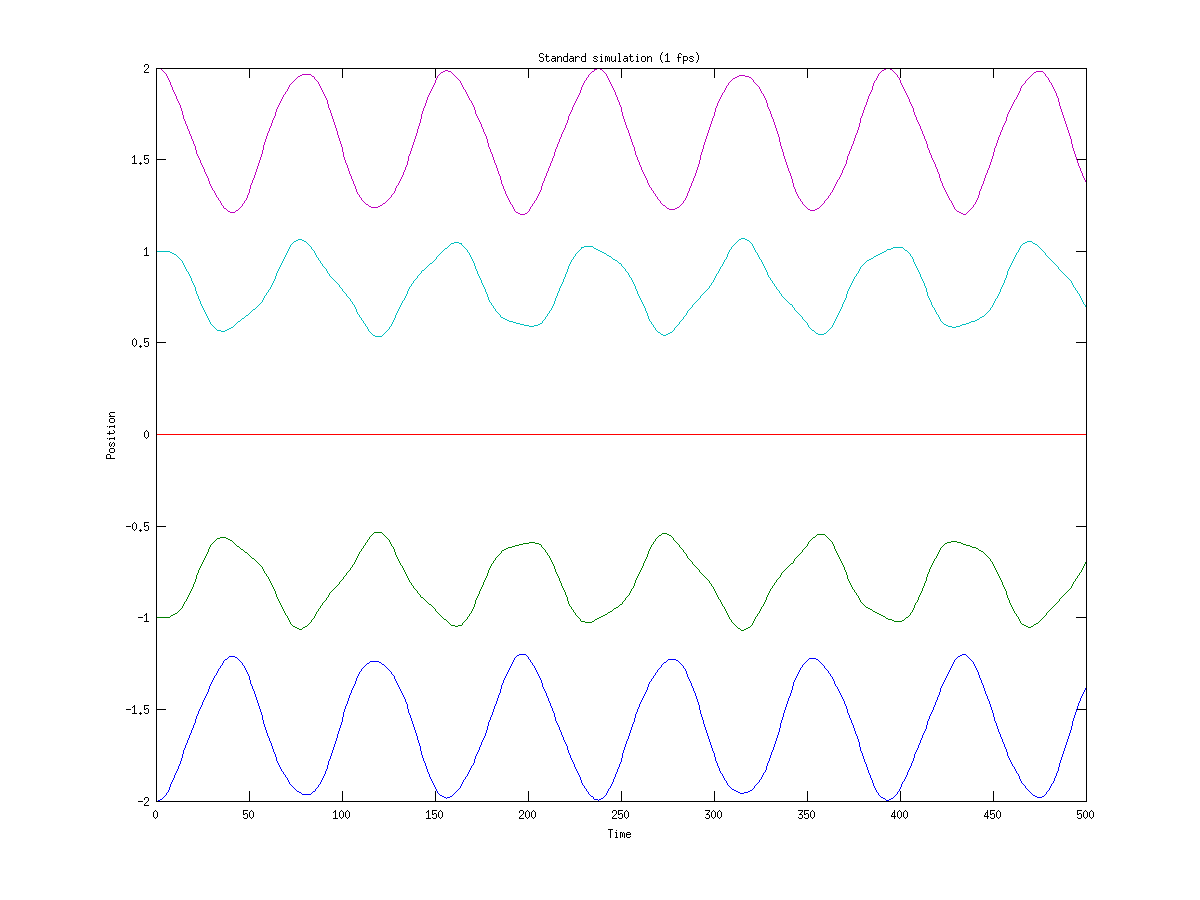
\includegraphics[width=\textwidth]{../images/standard_uniform_1fps.png}
        \caption{1 fps}
        \label{fig:std_uni_1fps}
    \end{subfigure}
    \caption{Standard simulations of particles distributed uniformly using
    different timestep sizes}
\end{figure}

\subsection{Adapt-on-switch}
Special things to note: How subdivision is done: new fixed (30) or relative (dt / 10)
new fixed: We don't catch it early enough. Maybe something with the explicit
euler, maybe something with the linear model. We should catch the error before
it escalates into a state in which we cannot rescue it anymore.

Relative: We get too fine-grained - maybe related to the above
\begin{figure}[H]
    \begin{subfigure}{0.5\textwidth}
        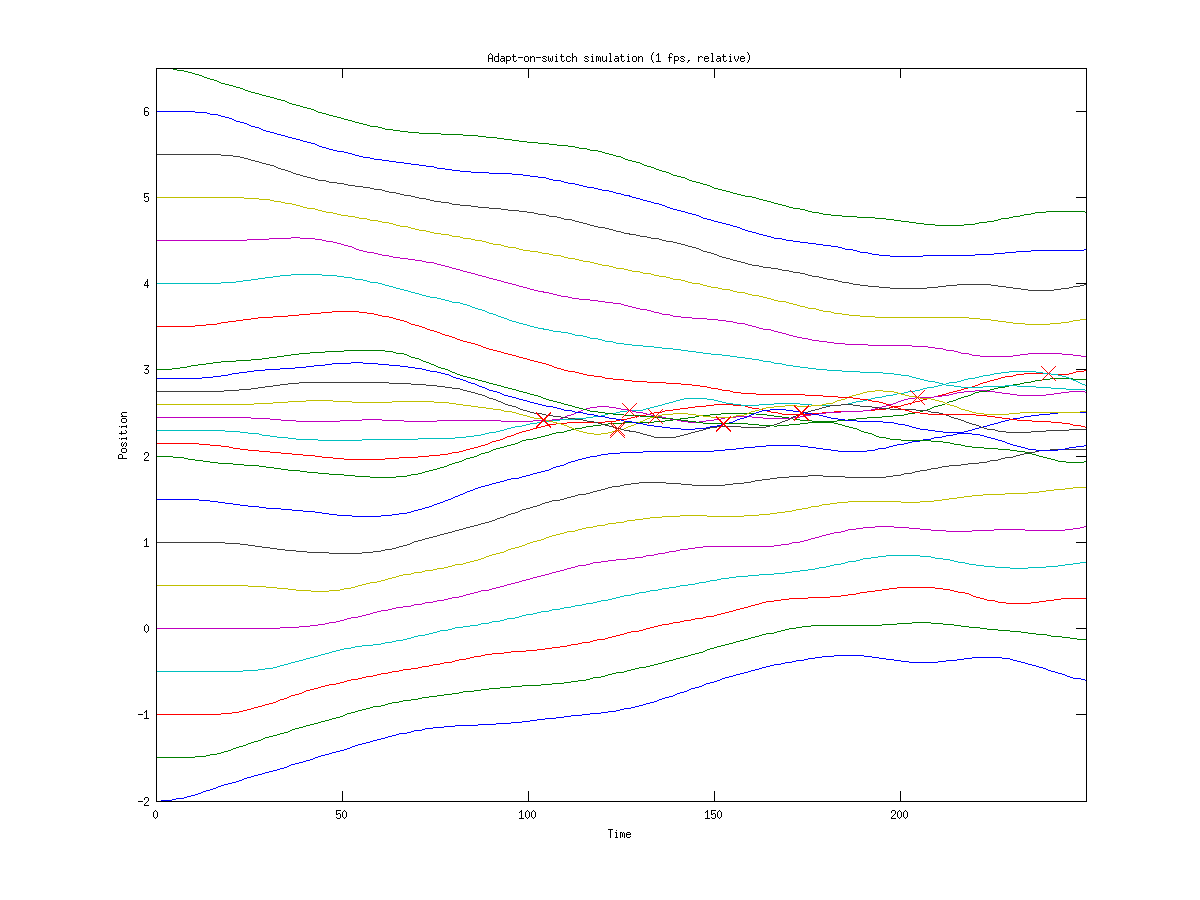
\includegraphics[width=\textwidth]{../images/switch_multiscale_1fps_relative.png}
        \caption{Relative timestepping ($\Delta t = \frac{\Delta t}{100}$)}
        \label{fig:switch_multi_1fps_relative}
    \end{subfigure}
    \begin{subfigure}{0.5\textwidth}
        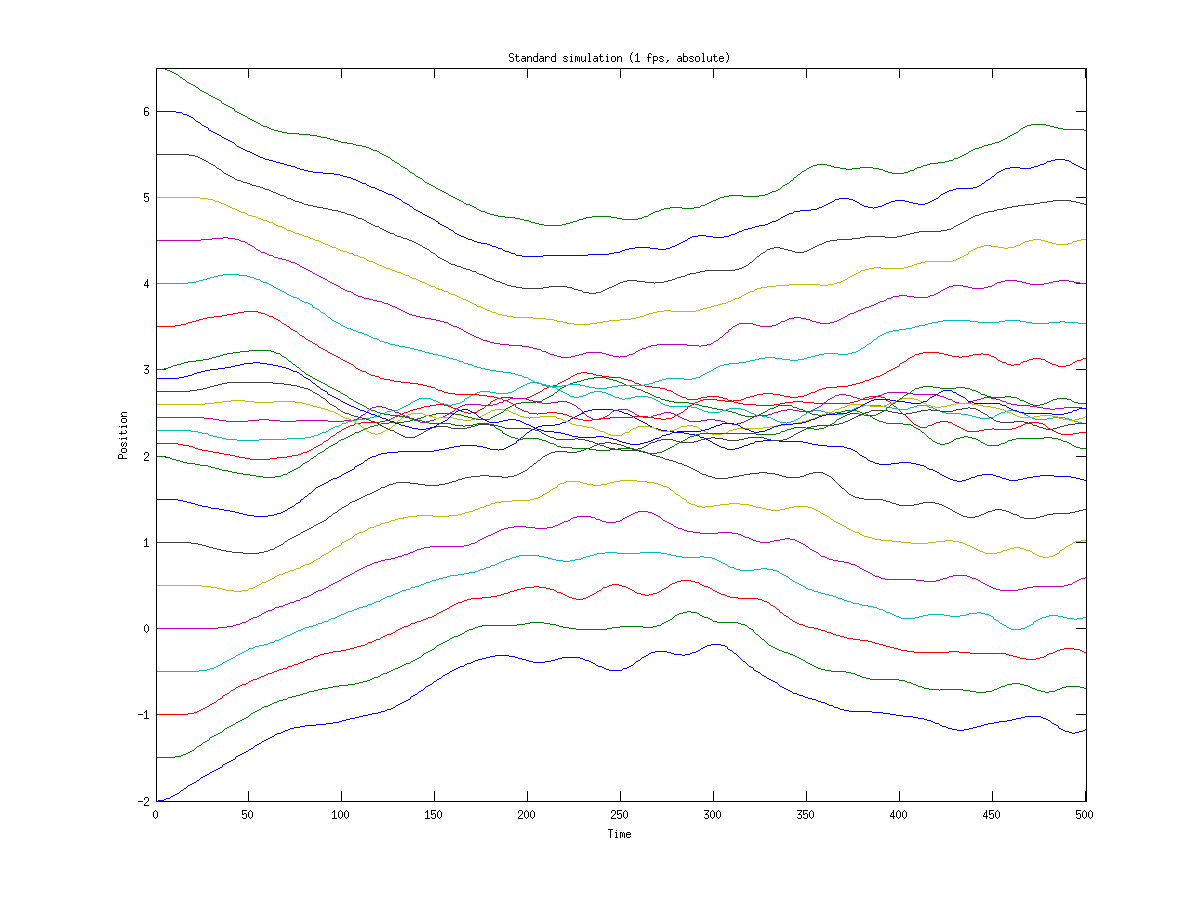
\includegraphics[width=\textwidth]{../images/switch_multiscale_1fps_absolute.png}
        \caption{Absolute timestepping ($\Delta t = \frac{1}{30}$)}
        \label{fig:switch_multi_1fps_absolute}
    \end{subfigure}
    \caption{Adapt-on-switch simulation of particles distributed with two
    scales using 1 fps}
\end{figure}

\subsection{Atomic updating using heuristics}

Heuristic: steps since last update and ratio of length since last update

interpolation of positions makes the integration more stable since the stepping
is based on a point closer in time

\subsection{Global estimated acceleration}

The heuristic dampens the system


%Examples of
%
%\begin{table}[H]
%\caption{Example table}
%\centering
%\begin{tabular}{llr}
%\toprule
%\multicolumn{2}{c}{Name} \\
%\cmidrule(r){1-2}
%First name & Last Name & Grade \\
%\midrule
%John & Doe & $7.5$ \\
%Richard & Miles & $2$ \\
%\bottomrule
%\end{tabular}
%\end{table}

%------------------------------------------------

\section{Discussion}

Adaptive timestepping based on highest acceleration/smallest grid
Relate to hyperelastic materials (some linear heuristic = win)

%----------------------------------------------------------------------------------------
%	REFERENCE LIST
%----------------------------------------------------------------------------------------

\section{Conclusion}

\bibliography{bibliography}
\bibliographystyle{plain}

%----------------------------------------------------------------------------------------


\end{document}
